\begin{frame}
\frametitle{Problem}
\textbf{Problems arising during packet capturing:}
\begin{itemize}
	\item High bit rates and packet rates
		\begin{itemize}
			\item [$\Rightarrow$] \textcolor{red}{high CPU load and packet loss} \newline
		\end{itemize}
\end{itemize}
\begin{figure}[H] 
	\subfigure{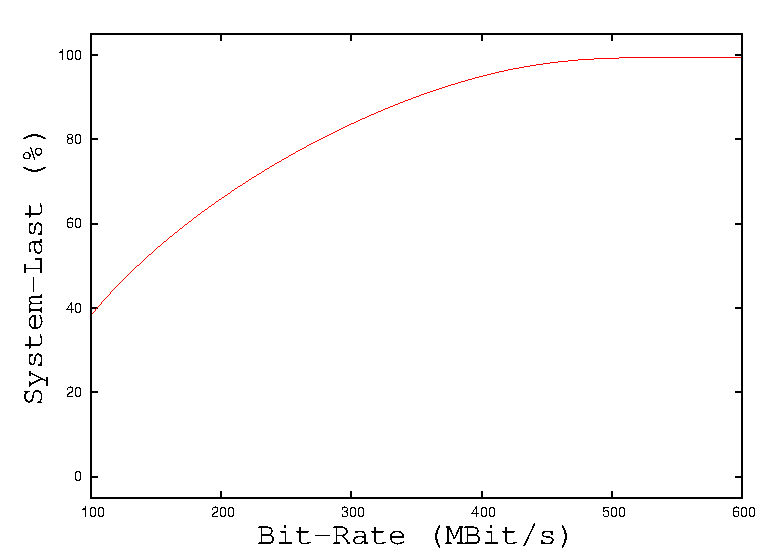
\includegraphics [width=0.45\textwidth]{plots/sysload_generic_slide}}
	\subfigure{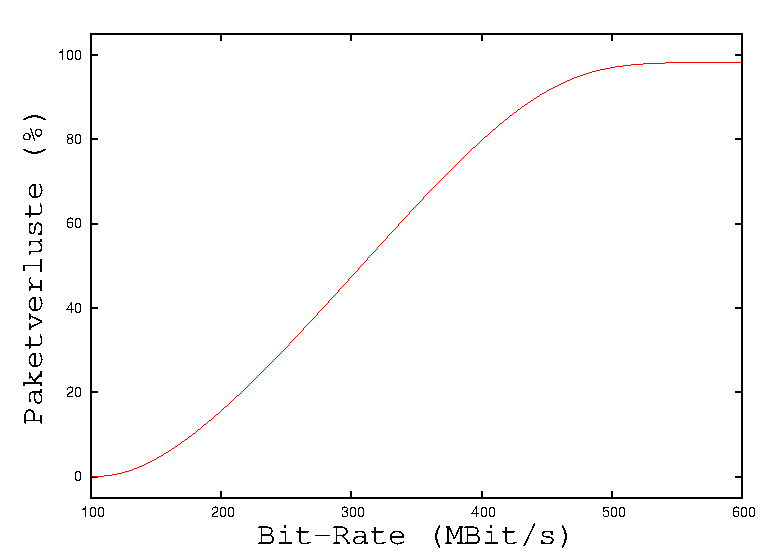
\includegraphics [width=0.45\textwidth]{plots/pktlos_generic_slide}}
	\caption{Capturing 64-Bytes packets. (Bezier curves)}
\end{figure}
\end{frame}

\begin{frame}
\frametitle{The reason of the Problems}
\textbf{Inefficiency of standard capturing software}\newline
\begin{itemize}
	\item To many ``expensive'' operations in terms of CPU cycles: 
\begin{itemize}
			\item System calls
			\item Packet copy operations
			\item Memory allocations
			\item etc\ldots\newline
\end{itemize}
% \begin{small}
% 	\item [$\Rightarrow$] probably the capturing software for FreeBSD was
% 		developed at a time when  network data-rates were low enough relative
% 		to hardware processing resources such that capturing loss problems did
% 		not arise?
% \end{small}
\end{itemize}
\end{frame}

